\documentclass{homework}
\usepackage{lipsum}
\usepackage{cancel}
\usepackage{amsthm}
\usepackage{cleveref}
\usepackage{upgreek}
\usepackage[framed]{mcode}
\usepackage{mathrsfs}
\usepackage{tikz}
\usepackage{units}
\usetikzlibrary{matrix}
\newtheorem{lemma}{Lemma}
\DeclareMathOperator*{\argmin}{arg\,min}

\title{Kevin Joyce}
\course{Math 514 - Inverse Problems - Homework 6}
\author{Kevin Joyce}
\docdate{\today}
\begin{document} 
\newcommand{\figref}[1]{\figurename~\ref{#1}}
\renewcommand{\bar}{\overline}
\renewcommand{\hat}{\widehat}
\renewcommand{\SS}{\mathcal S}
\newcommand{\HH}{\mathscr H}
\newcommand{\mom}{\widetilde}
\newcommand{\mle}{\widehat \Uptheta}
\newcommand{\eps}{\varepsilon}
\newcommand{\todist}{\stackrel{D}\longrightarrow}
\newcommand{\toprob}{\stackrel{p}\longrightarrow}
\newcommand{\TTheta}{\overline{\underline \Theta} }
\newcommand{\del}{\partial}
\newcommand{\approxsim}{\overset{\cdotp}{\underset{\cdotp}{\sim}}}

Codes for each problem are available at \url{https://github.com/kjoyce/inverse_problems/tree/master/homework04/codes}

\problem{Bardsley 3.14. Modify \texttt{Tomography.m} so that it implements Kaczmarz's Method.  How many sweeps through all of the indicies, i.e. implementations of the method, does it take to obtain a good reconstruction? }

\begin{solution}
Adding the following lines of code implements the method.  We ues the DP stopping criterion to determine the amount of iterations.

\begin{minipage}{.4\textwidth}
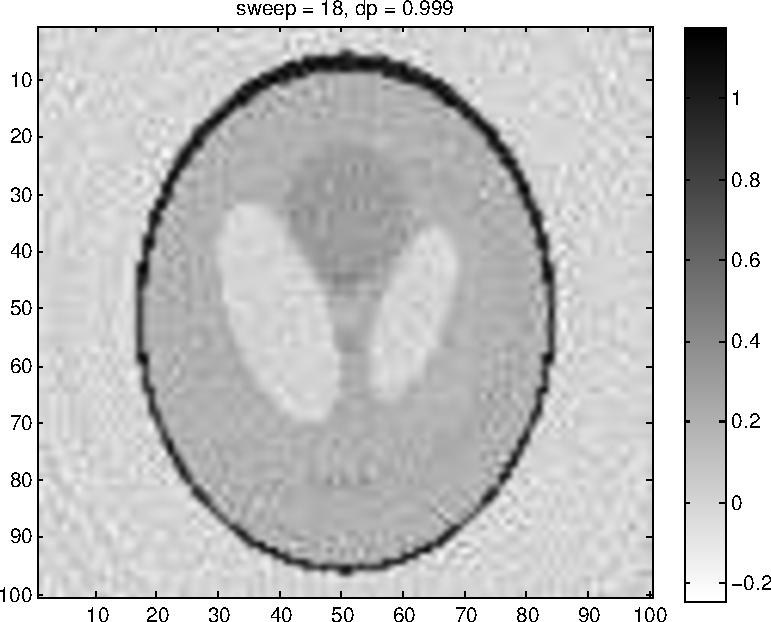
\includegraphics[width=\textwidth]{tomography.pdf}
\end{minipage}
\begin{minipage}{.55\textwidth}
\begin{lstlisting}
x = A(1,:)';
i = 1;
while 1
  i = i + 1;
  x  = x + (b(i) - A(i,:)*x)/norm(A(i,:))^2 * A(i,:)';
  dp = norm( A*x - b(:) )/(size(A,1)*noise^2);
  if i == size(A,1)
    i = 0;
  end
  if dp <= 1
    break
  end
end 
\end{lstlisting}
\end{minipage}

\end{solution}

\renewcommand{\NN}{\ensuremath{\mathcal N}}
\begin{longproblem} Bardsley 4.3. Sampling from Gaussian probability densities.  

  \subproblem{ Let $\vect B$ be an $m\times n$ matrix, $\vect v \sim \NN(\vect \mu,\vect C)$, and $\vect w = \vect{Bv}$, then $\vect w \sim \NN(\vect{B\mu}, \vect{BCB}^T)$.$^\dagger$  Use this to show that if $\vect R$ is a square root matrix for $\vect C$, i.e. $\vect C = \vect R^T\vect R$, and if $\vect v\sim \NN(\vect 0,\vect I)$ then $\vect w = \vect \mu +\vect R^T\vect v$ has distribution $\vect w \sim \NN(\vect \mu,\vect C)$.}

  By linearity, $E[ \vect w ] = \vect \mu + \vect R^T \vect 0 = \vect \mu$, and by $\dagger$, $Var[ \vect w] = \vect R^T\vect{IR} = \vect C$.
  
  \subproblem{ Use MATLAB and part (a) to compute and plot 1000 samples from the random vector $\ds{\vect w \sim \NN\left(\begin{bmatrix}1\\1\end{bmatrix}, \begin{bmatrix}2&-1\\-1&2\end{bmatrix}\right)}$.}

\begin{minipage}{.4\textwidth}
  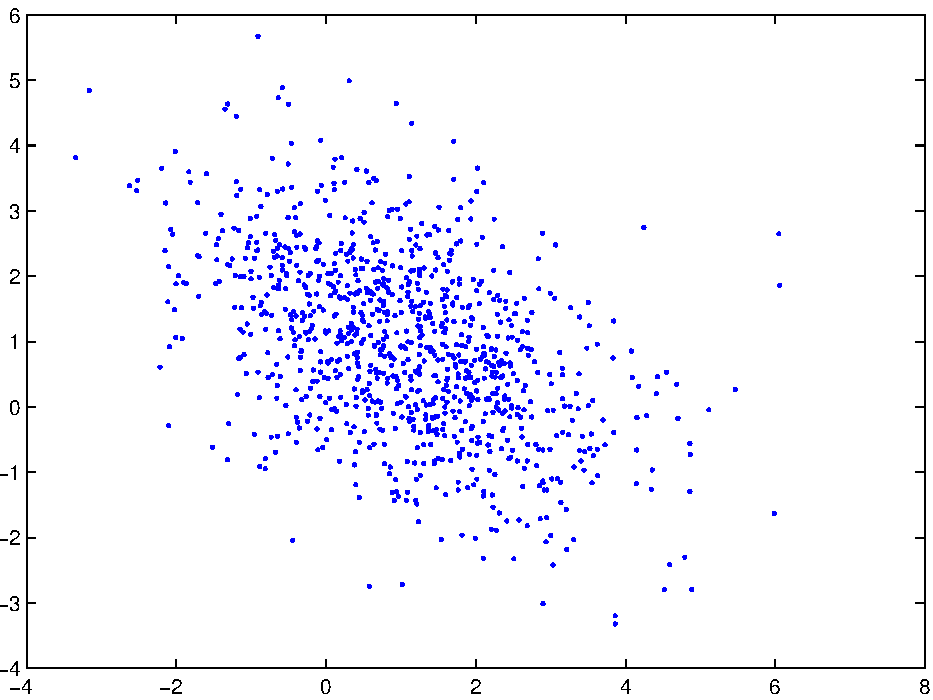
\includegraphics[width=\textwidth]{samples.pdf}
\end{minipage}
\begin{minipage}{.55\textwidth}
\begin{lstlisting}
n = 1000
v = randn(2,n);
mu = ones(2,n);
C = [2 -1;-1 2];
R = chol(C);
w = mu + R'*v;
plot(w(1,:),w(2,:),'.') ,xlim([-5,7]) ,ylim([-5,7]);
\end{lstlisting}
\end{minipage}

  \subproblem{ If $\vect v = (v_1,\dots,v_k)$ is a random vector such that $v_i \sim \NN(0,1)$ for $i = 1,\dots,k$, then $Q = \sum_{i=1}^k w_i^2$ is a $\chi^2(k)$ random variable.  Verify that, approximately, a correct amount of the sampled points from part (b) are located inside the confidence regions given by $95\%$ and $99\%$ limits of the $\chi^2(2)$ distribution, computed using the \texttt{chi2inv} funciton.  Note that you need to normalize the samples, i.e. look at $\vect C^{-1/2}(\vect \mu - \vect w_i)$.}

\begin{minipage}{.4\textwidth}
  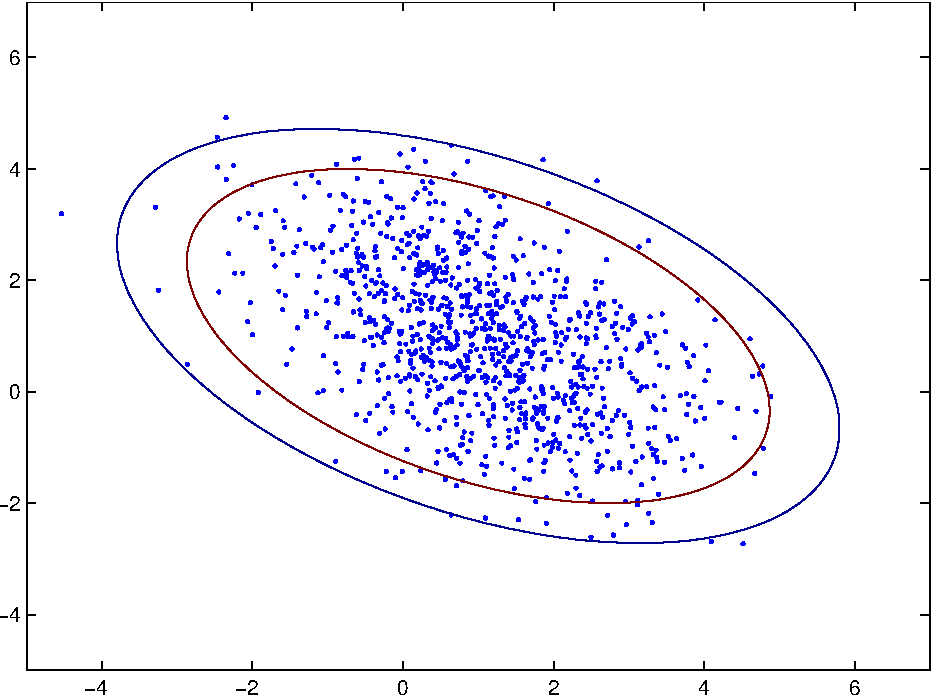
\includegraphics[width=\textwidth]{conf_ellipse.pdf}
\end{minipage}
\begin{minipage}{.55\textwidth}
\begin{lstlisting}
vv = R\(w - mu);
xi = sum(vv.^2);
alpha = .05;
l1 = chi2inv((1-alpha),2);
alpha = .01;
l2 = chi2inv((1-alpha),2);
sum(xi <= l1)/length(xi)
ans =

    0.9490

sum(xi <= l2)/length(xi)
ans =

    0.9920

\end{lstlisting}
\end{minipage}

\end{longproblem}

\begin{longproblem}
  Bardsley 4.4. GMRF with periodic boundary conditions.

  Modify \texttt{GMRFDirichlet.m} so that it computes samples from
  (4.16) where $\vect L_{1D}$ is given by (4.17) in one dimension
  and (4.14) in two dimensions.  Note that these precision matrices
  have a zero eigenvalue, so you cannot use the Cholesky
  factorization.  Instead, Compute the square root of $\vect L$ and $\vect
  L^\dagger$ using an eigenvalue decomposition.  To compute the eigen values decomposition in two dimensions, note that multiplication by $\vect L_{2D}$ is equivalent to discrete convolution with the $n\times n$ kernel
  $$
    \vect l = \begin{bmatrix}
      l_{-n/2,n/2-1} & \cdots & l_{0,n/2-1} & \cdots & l_{n/2-1,n/2-1} \\
      \vdots & \ddots & \vdots & \ddots & \vdots \\
      l_{-n/2,0} & \cdots & l_{0,0} & \cdots & l_{n/2-1,0} \\
      \vdots & \ddots & \vdots & \ddots & \vdots \\
      l_{-n/2,-n/2} & \cdots & l_{0,-n/2} & \cdots & l_{n/2-1,-n/2} \\
    \end{bmatrix},
  $$
  where $l_{0,0} = 4$, $l_{-1,0} =l_{1,0} =l_{0,-1} =l_{0,1} = -1$
  and $l_{ij} = 0$ otherwise.  The periodic boundary condition makes
  $\vect L_{2D}$ a BCCB matrix with eigenvalues $\vect{\hat l_s} = n \mathrm{DFT}(\vect l_s)$, where $\vect l_s = \texttt{fftshift}(\vect l)$, and that 
  $ \vect{Lx} = \mathrm{vec} \Big(\mathrm{IDFT}(\vect{\hat l_s} \odot \mathrm{DFT}(\vect X)\Big)
  $.

  Use this factorization, and the corresponding factorization for $\vect L^\dagger$, to compute samples in the two dimensional case.
\end{longproblem}

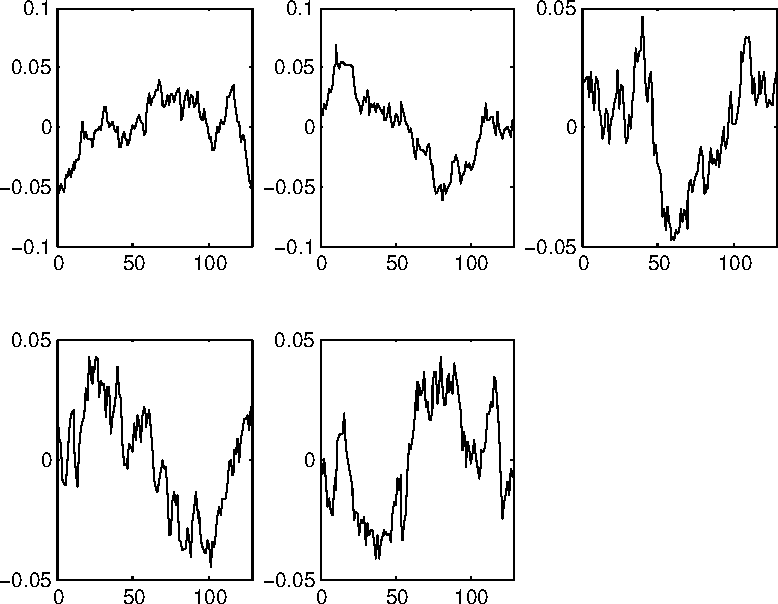
\includegraphics[width=.5\textwidth]{period_samps.pdf}
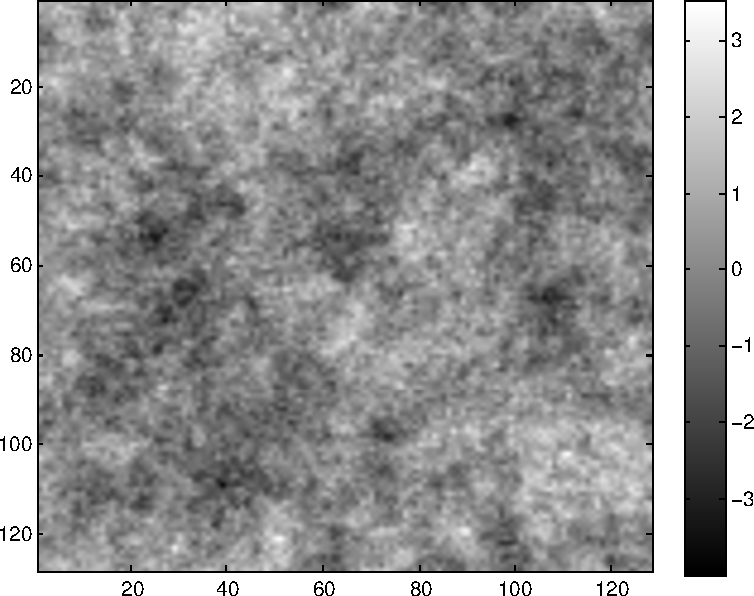
\includegraphics[width=.5\textwidth]{2dperiod_samps.pdf}

\end{document}
